%% The first command in your LaTeX source must be the \documentclass command.
%%
%% Options:
%% twocolumn : Two column layout.
%% hf: enable header and footer.
\documentclass[
% twocolumn,
% hf,
]{ceurart}

\setlength{\leftmargini}{8em} 

%%
%% One can fix some overfulls
\sloppy


%%%%% My macros
\usepackage[T1]{fontenc} % for pipe symbol |
\usepackage[utf8]{inputenc} % for french accents
\usepackage{ifthen}
\usepackage{graphicx}
\usepackage{hyperref}
\usepackage{multirow}
\usepackage{array} % for aligning table columns
\usepackage{arydshln} % for dashed lines in tables
\usepackage[many]{tcolorbox} % for bordered theorem boxes

\usepackage{xspace}
\usepackage{xcolor}
\usepackage[normalem]{ulem} 			% \sout macro
\usepackage{amsmath,amsfonts}

\usepackage{caption} % for subfigures
\usepackage{subcaption} % for subfigures

\newcolumntype{L}[1]{>{\raggedright\let\newline\\\arraybackslash\hspace{0pt}}p{#1}}
\newcolumntype{C}[1]{>{\centering\let\newline\\\arraybackslash\hspace{0pt}}p{#1}}
\newcolumntype{R}[1]{>{\raggedleft\let\newline\\\arraybackslash\hspace{0pt}}p{#1}}

\newboolean{showcomments}
\setboolean{showcomments}{true}
% \setboolean{showcomments}{true}


% ********************************************************************* 
% Revisions and comments Macros
% ********************************************************************* 
	
\ifthenelse{\boolean{showcomments}}
{
	\newcommand{\nb}[3]{
		{\colorbox{#2}{\bfseries\sffamily\scriptsize\textcolor{white}{#1}}}
		{\textcolor{#2}{\sf\small$\blacktriangleright$\textit{#3}$\blacktriangleleft$}}}
	 \newcommand{\version}{\emph{\scriptsize$-$Id$-$}}
	\newcommand{\bnote}[2]{\fbox{\color{blue}\bfseries\sffamily\scriptsize#1}
    	{\color{blue}\sf\small$\blacktriangleright$\textit{#2}$\blacktriangleleft$}}
	\newcommand{\old}[1]{{\color{gray}\sout{#1}}} % old to be removed
	\newcommand{\del}[1]{\old{#1}} % please remove
	\newcommand{\ins}[1]{{\textcolor{blue}{\uline{#1}}}} % please insert	
	\newcommand{\ugh}[1]{{\textcolor{red}{\uwave{#1}}}} % please rephrase	
	\newcommand{\chg}[2]{{\textcolor{red}{\sout{#1}}}{\ra}\textcolor{blue}{\uline{#2}}} % please change
	\newcommand{\here}{\bnote{***}{CONTINUE HERE}} 
	\newcommand{\fix}[1]{\bnote{FIX}{#1}}
}{
	\newcommand{\bnote}[2]{}
	\newcommand{\nb}[3]{}
	\newcommand{\old}[1]{}
	\newcommand{\del}[1]{}
	\newcommand{\ins}[1]{}
	\newcommand{\ugh}[1]{}
	\newcommand{\chg}[2]{}
	\newcommand{\here}{}
	\newcommand{\fix}[1]{}
} 

\newcommand{\hide}[1]{}




%---% add your own macros 
\newcommand{\np}[1]{\nb{palumbon}{orange}{#1}}
\newcommand{\sd}[1]{\nb{Stephane}{red}{#1}}
\newcommand{\sj}[1]{\nb{Sebas}{teal}{#1}}
\newcommand{\sebas}[1]{\nb{Sebas}{teal}{#1}}
\newcommand{\gp}[1]{\nb{Guille}{violet}{#1}}
%olive
%---





\graphicspath{{figures/}{newFigures/}}
%%% 


\newcommand{\figref}[1]{Figure~\ref{fig:#1}}
\newcommand{\figlabel}[1]{\label{fig:#1}}
% \newcommand{\tabref}[1]{Table~\ref{tab:#1}}
\newcommand{\layout}[1]{#1}
\newcommand{\commented}[1]{}
\newcommand{\secref}[1]{Section \ref{sec:#1}}
\newcommand{\appref}[1]{Appendix \ref{sec:#1}}
\newcommand{\seclabel}[1]{\label{sec:#1}}

%\newcommand{\ct}[1]{\textsf{#1}}
\newcommand{\stCode}[1]{\textsf{#1}}
\newcommand{\stMethod}[1]{\textsf{#1}}
%\newcommand{\sep}{\texttt{>>}\xspace}
\newcommand{\stAssoc}{\texttt{->}\xspace}

\newcommand{\stBar}{$\mid$}
\newcommand{\stSelector}{$\gg$}
\newcommand{\ret}{\^{}}
\newcommand{\msup}{$>$}
%\newcommand{\ret}{$\uparrow$\xspace}

\newcommand{\myparagraph}[1]{\noindent\textbf{#1.}}
\newcommand{\eg}{\emph{e.g.,}\xspace}
\newcommand{\ie}{\emph{i.e.,}\xspace}
\newcommand{\etal}{\emph{et al.,}\xspace}
\newcommand{\ct}[1]{{\textsf{#1}}\xspace}


\newenvironment{code}
    {\begin{alltt}\sffamily}
    {\end{alltt}\normalsize}

\newcommand{\defaultScale}{0.55}
\newcommand{\pic}[3]{
   \begin{figure}[h]
   \begin{center}
   \includegraphics[scale=\defaultScale]{#1}
   \caption{#2}
   \label{#3}
   \end{center}
   \end{figure}
}

\newcommand{\twocolumnpic}[3]{
   \begin{figure*}[!ht]
   \begin{center}
   \includegraphics[scale=\defaultScale]{#1}
   \caption{#2}
   \label{#3}
   \end{center}
   \end{figure*}}

\newcommand{\infe}{$<$}
\newcommand{\supe}{$\rightarrow$\xspace}
\newcommand{\di}{$\gg$\xspace}
\newcommand{\adhoc}{\textit{ad-hoc}\xspace}

\usepackage{url}            
\makeatletter
\def\url@leostyle{%
  \@ifundefined{selectfont}{\def\UrlFont{\sf}}{\def\UrlFont{\small\sffamily}}}
\makeatother
% Now actually use the newly defined style.
\urlstyle{leo}

% --- Defining boxes (tcolorbox)
\definecolor{main}{HTML}{828282}    % setting main color to be used
\definecolor{sub}{HTML}{E0E0E0}     % setting sub color to be used

\tcbset{
    sharp corners,
    colback = white,
    before skip = 0.2cm,    % add extra space before the box
    after skip = 0.5cm      % add extra space after the box
}                           % setting global options for tcolorbox

\newtcolorbox{cbox}{
    enhanced, % for a fancier setting,
    boxrule = 0pt, % clearing the default rule
    borderline = {0.75pt}{0pt}{main}, % outer line
    borderline = {0.75pt}{2pt}{sub} % inner line
}

% syntax highlighting for Pharo in code blocks
\include{./smalltalkEnv}


%%
%% Minted listings support 
%% Need pygment <http://pygments.org/> <http://pypi.python.org/pypi/Pygments>
\usepackage{listings}
\usepackage{algorithmic}
\usepackage{graphicx}
\usepackage{textcomp}
\usepackage{xcolor}
\usepackage{multirow}
\usepackage{multicol}





%%
%% end of the preamble, start of the body of the document source.
\begin{document}

%%
%% Rights management information.
%% CC-BY is default license.
\copyrightyear{2026}
\copyrightclause{Copyright for this paper by its authors.
  Use permitted under Creative Commons License Attribution 4.0
  International (CC BY 4.0).}

%%
%% This command is for the conference information
\conference{IWST 2026: International Workshop on Smalltalk Technologies, July 4--10, 2026, Plovdiv, Bulgaria}

%%
%% The "title" command
\title{Phizura: On-the-Fly Music Recording with Method Proxies}



%%
%% The "author" command and its associated commands are used to define
%% the authors and their affiliations.
\author[1]{Domenico Cipriani}[%
orcid=0009-0005-3023-3192,
email=mspgate@gmail.com,
]


\author[2]{Sebastian {Jordan Montaño}}[%
orcid=0000-0002-7726-8377,
email=sebastian.jordan@inria.fr,
% orcid=0000-0002-7726-8377,
% url=https://jordanmontt.fr,
]

\author[2]{Stéphane Ducasse}[
orcid=0000-0001-6070-6599,
email=stephane.ducasse@inria.fr,
]

\address[1]{Evref,  Inria, CNRS, Centrale Lille, UMR 9189 CRIStAL, Park Plaza, Parc scientifique de la Haute-Borne, 40 Av. Halley Bât A, 59650 Villeneuve-d’Ascq, France}
\address[2]{Univ. Lille, Inria, CNRS, Centrale Lille, UMR 9189 CRIStAL, Park Plaza, Parc scientifique de la Haute-Borne, 40 Av. Halley Bât A, 59650 Villeneuve-d’Ascq, France}


%%
%% The abstract is a short summary of the work to be presented in the
%% article.
\begin{abstract}
Live coding is a performance practice in which artists write and modify code in real time to generate music. A key challenge is capturing a performance for later replay, sharing, or analysis without resorting to audio recording. This paper presents Phizura, a recording tool for on-the-fly music performances conducted with Coypu, a Pharo-based library and dialect for live music programming. Phizura leverages Method Proxies, a safe and fast message-passing control library, to non-intrusively intercept Playground evaluations and keystrokes during a performance. The recorded data, timestamped expressions and input events, can later be emitted as executable Pharo code that faithfully replays the performance with the original timing. We describe the architecture of Phizura, detail how Method Proxies enable a clean separation between recording logic and the Coypu codebase, and compare the approach to a previous Announcer-based implementation.
\end{abstract}

%%
%% Keywords. The author(s) should pick words that accurately describe
%% the work being presented. Separate the keywords with commas.
\begin{keywords}
  Pharo\sep
  Method Proxies \sep
  Coypu \sep
  On-the-fly music programming
\end{keywords}

%%
%% This command processes the author and affiliation and title
%% information and builds the first part of the formatted document.
\maketitle



\section{Introduction}\label{sec:intro}
Live coding is an increasingly popular creative practice in which performers write and modify source code in real time to produce music, visuals, or other time-based media\footnote{TOPLAP Manifesto at \url{https://toplap.org/wiki/ManifestoDraft}}.
The field has developed a substantial academic presence: the International Conference on Live Coding (ICLC), now in its tenth year, has served as the primary venue for peer-reviewed research on the practice, attracting contributions from computer science, music, and the performing arts.
Programming languages such as Tidal Cycles\cite{McLe14}, Sonic Pi\cite{Aar16}, and Orca\cite{Mess21} have popularized the practice, each offering alternative syntaxes and notations for expressing musical patterns. Within the Pharo ecosystem, Coypu\cite{Cipr25c} provides a library and a DSL for on-the-fly music programming, enabling performers to construct rhythmic sequences, melodic patterns, and to modify them interactively in a Playground.

To date, relatively little scholarly attention has been devoted to capturing and preserving live coding performances, particularly the generative process itself. Audio recording captures the sonic result but discards the compositional process: the sequence of code edits, evaluations, and their precise timing. Audio files are also large, difficult to share, and impossible to re-execute under a different setup. Compositional data, by contrast, enables exact replay of a performance with alternative sound synthesis, facilitates sharing between musicians as lightweight text files, supports analysis of live coding practice, and opens the door to automated post-processing of performances. This concern has been raised explicitly in the Tidal Cycles community\footnote{Tidal Club Forum, How to replay a live coding session. Link at \url{https://club.tidalcycles.org/t/how-to-replay-a-live-coding-session/464}, 2020.}, where users have discussed the need for tools that store every evaluation with its timestamp and allow session-based replay. However, no integrated solution has emerged so far.

This paper presents the design and implementation of Phizura, shows how Method Proxies\cite{Jord24b} can be applied beyond profiling and debugging to support creative coding workflows, and compares the current approach to the previous Announcer-based implementation. The paper begins with background on Coypu and Method Proxies, then discusses the limitations of the earlier Announcer-based approach that motivated the redesign. It continues with the architecture and implementation of Phizura, the code emission and replay mechanism, and a discussion of related work. It closes with a reflection on generality, limitations, and future directions.


\section{Background}\label{sec:bac}

\subsection{Live coding}

Pienso que es importante que empecemos hablando de live coding. Que el enfoque del paper sea más del lado de live coding y que el público sea informáticos que no conoces mucho sobre live coding.

\subsection{Coypu: programming music on-the-fly with Pharo}

\sebas{Para conectar esta parte con el live coding; sería también hablar de como se usa Coypu para hacer live coding. Entonces esta subsection tendría tres partres: primero como Coypu se usa para livecoding; después que Coypu se usa en el Playground}
Coypu\cite{Cipr25c} is a library and domain-specific dialect for live music programming within the Pharo environment. It acts as a client for an audio server, which can be either internal (a Phausto\cite{Cipr24b} DSP running within Pharo) or an external OSC-capable\footnote{Open Sound Control (OSC) is a protocol for real-time communication between multimedia devices and software, typically transmitted over UDP, \url{https://opensoundcontrol.stanford.edu}.}application, typically SuperCollider via the SuperDirt engine, or a MIDI device.
A performer works in a Pharo Playground, writing expressions that define rhythmic and melodic patterns and assign them to named instruments. Once evaluated, these patterns begin playing immediately. From that point on, the performer reshapes the music in real time: modifying patterns, muting or soloing individual voices, swapping instruments, and layering new material over what is already running. Every evaluation hits the running output immediately. The performance is shaped by what gets evaluated, when, and in what order and that is exactly what Phizura records.
\sebas{Sería bueno poner una figura que muestra el live coding. Puede ser una foto, una screenshot. Y también estaría bueno poner como pie de nota un video de youtube de livecoding}

\subsection{Method Proxies: safe and fast method interception}

MethodProxies~\cite{Jord24b} is a per-method instrumentation library for Pharo that implements \emph{message-passing control}: an instrumentation paradigm in which user-defined code can be executed \emph{before}, \emph{after}, or \emph{instead of} a method invocation, as well as during the stack unwind triggered by an exception or non-local return.
\textbf{It leaves the source code of the instrumented application intact.}
The library exposes a stratified architecture in which the user-facing API is reduced to subclassing a handler class (\ct{MpHandler}) and overriding a small set of hooks; the framework manages the underlying instrumentation mechanics. The same handler can be associated with several proxied methods, which allows information to be aggregated across distinct call sites without duplicating logic.

Internally, each instrumented method is replaced in its method dictionary by a precompiled \emph{trap method} that orchestrates the execution of the hooks. To avoid runtime compilation, MethodProxies ships a small set of precompiled trap prototypes --- one per method arity --- that are copied at installation time and patched with three literals: the handler, the deactivator used to react to stack unwinds, and the selector under which the original method is re-installed as a hidden entry of the same method dictionary. Because the trap remains a regular \ct{CompiledMethod}, it is JIT-compiled by the virtual machine and the forwarding send to the original becomes monomorphic, which keeps the per-call overhead low. Stack unwinds are handled through the VM's built-in unwind mechanism rather than through the standard \ct{ensure:} construct, avoiding the allocation of block closures and the associated stack reification cost.

MethodProxies also guarantees a number of properties that make it suitable for instrumenting arbitrary parts of the system, including the language kernel. It is \emph{meta-safe} --- instrumented methods can be invoked from within a handler without re-entering the instrumentation, since the active process is marked as meta-level during hook execution and the trap is bypassed while this flag is set.
It is \emph{unwind-safe}, supports dynamic installation and deinstallation at run time, and reports an average overhead of approximately 1.5~$\times$ with the meta-safety mechanism itself adding only about 9\%~\cite{Jord24b}.

\subsection{Previous approaches to capturing performances}
The first recording mechanism for Coypu was implemented by Redwane Engels during an internship and demonstrated at ESUG 2024 in Lille.
It relied on Pharo's \texttt{Announcer} and \texttt{Announcement} classes, which implement the observer design pattern.

The approach was straightforward: the Coypu codebase itself was modified so that at each point where an evaluation could produce a musical effect, an announcement was explicitly fired.
A subscriber object, the recorder, registered interest in these announcements and logged each one with a timestamp.

It functioned as intended, but introduced significant trade-offs.
Recording logic was distributed throughout the codebase, and supporting each new recordable event required direct modifications to the source code.
The recorder depended on specific announcement classes defined within the library, making the two systems difficult to evolve independently.
Extending it to capture additional events, such as keystrokes, cursor positions, or events from other tools, required yet more invasive changes.
And every modification to the evaluation pipeline risked breaking or silently bypassing the recording hooks.
These limitations motivated the redesign using Method Proxies, which externalizes the instrumentation entirely and it does not require modifying the source code.

\section{Design and Implementation}

Phizura is organized in three packages: \texttt{Phizura} (core recording and emission logic), \texttt{Phizura-Playground} (UI integration), and \texttt{Phizura-Tests} (test suite). The architecture addresses four concerns: instrumentation, recording, code emission, and UI integration.

\subsection{Instrumentation}

At the core of Phizura's design is a small class hierarchy for instrumentation. \texttt{PhizuraInstrumentor} is an abstract class that manages a collection of \texttt{MpMethodProxy} instances and a shared \texttt{PhizuraHandler}. Subclasses define which methods to instrument by implementing \texttt{initializeMethodProxies}.

\begin{lstlisting}[label={lst:instrumentor-initialize},caption={Initialization of PhizuraInstrumentor}]
PhizuraInstrumentor >> initialize
    super initialize.
    instrumentationHandler := PhizuraHandler
        onRecorder: recorder.
    self initializeProxyVariables.
    self initializeMethodProxies
\end{lstlisting}

The concrete subclass \texttt{PhizuraEvaluationInstrumentor} instruments two methods: \texttt{SpCodeSelectionCommand>>\#evaluate:andDo:}, the standard Pharo Playground evaluation command, and \texttt{PhizuraPlaygroundPagePresenter>>\#doEvaluateAndGoFor:}, the Phizura Playground's own evaluation path. Both share the same handler instance, so all evaluations are recorded uniformly regardless of which path triggers them.

The handler itself, \texttt{PhizuraHandler}, is a subclass of \texttt{MpHandler} and constitutes the only user-defined hook in the entire system. It implements a single method:

\begin{lstlisting}[label={lst:handler-before},caption={PhizuraHandler before-execution hook}]
PhizuraHandler >> beforeExecutionWithReceiver:
    anObject arguments: anArrayOfArguments
    | argument |
    argument := anArrayOfArguments first.
    recorder addRecord:
        (PhizuraEvaluationRecordEntry new
            time: DateAndTime now;
            expression: argument;
            cursorPosition:
                playgroundPage text cursorPosition;
            yourself)
\end{lstlisting}

The handler extracts the first argument of the intercepted method, which is the expression string being evaluated, and creates a record entry with three pieces of information: the current timestamp, the expression text, and the cursor position in the editor. No Coypu method is modified, subclassed, or even referenced. The instrumentation is purely additive.

\subsection{Recording}

Phizura captures two kinds of events, modeled by a small class hierarchy rooted at \texttt{PhizuraBasicRecordEntry}. \texttt{PhizuraEvaluationRecordEntry} stores a code expression, a timestamp, and the cursor position, corresponding to Playground evaluations. \texttt{PhizuraKeyEventRecordEntry} stores a keyboard key, a timestamp, and the cursor position, captured via a \texttt{whenKeyUpDo:} event handler on the Playground's text presenter, independently of Method Proxies. Both entry types participate in double dispatch for code emission (see Section~5).

\texttt{PhizuraRecorder} ties the system together. It holds a collection of record entries, a reference to the instrumentor, and a boolean recording flag. When \texttt{record} is called, it creates a \texttt{PhizuraEvaluationInstrumentor}, installs the proxies, and sets the flag. When \texttt{stopRecording} is called, it uninstalls all proxies. A guard \texttt{isRecording ifTrue:} ensures that evaluations outside a recording session are not captured. For emergency recovery, a class-side \texttt{forceUnrecord} method uninstalls all proxies in the image.

\subsection{The Phizura Playground}

Phizura requires a custom Playground to intercept the text that is evaluated when the user presses Cmd+D (Do it). The standard Pharo Playground does not expose the evaluated expression in a way that can be captured externally. The expression text flows through internal methods that are not designed for observation. To solve this, Phizura provides its own Playground, built by subclassing the standard Pharo Playground classes at four points.

\texttt{PhizuraPlaygroundPresenter}, a subclass of \texttt{StPlaygroundPresenter}, manages the window lifecycle. It ensures that recording stops when the window is closed and creates instances of \texttt{PhizuraPlaygroundPage} instead of the default page.

\texttt{PhizuraPlaygroundPagePresenter}, a subclass of \texttt{StPlaygroundPagePresenter}, is the central customization point. It defines the method \texttt{doEvaluateAndGoFor:}, which receives the selected text as its argument and evaluates it. This method is one of the two targets instrumented by Method Proxies, and it is where the handler intercepts the expression being evaluated. In addition, this presenter initializes the recorder, registers a \texttt{whenKeyUpDo:} event handler to capture keystrokes, sets up a custom interaction model via \texttt{PhizuraPlaygroundInteractionModel}, and extends the toolbar with five commands: \textit{Phizurear} (toggle recording), \textit{Clean Phizura} (reset the recorder), \textit{Inspect Phizura} (open an inspector on the recorder), \textit{Open MoofLOD} (emit code with OSC messages), and \textit{Open Records} (emit clean performance code).

\begin{figure}[ht!]
\begin{center}
   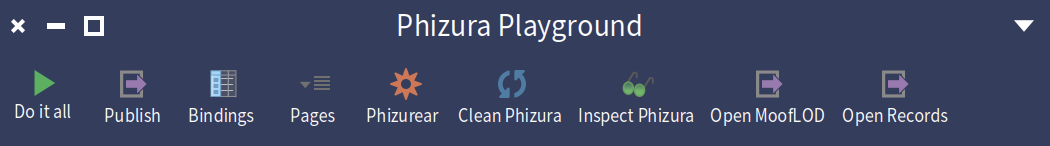
\includegraphics[width=0.75\linewidth]{assets/phizuraBar-screenshot.png}	
\end{center}
\caption{The Phizura Playground toolbar with the 5th extra commands.
\label{fig:phizuraPG-toolbar}}
\end{figure}

\texttt{PhizuraPlaygroundPage}, a subclass of \texttt{StPlaygroundPage}, overrides \texttt{defaultObjectInspectorClass} to return \texttt{PhizuraPlaygroundPagePresenter}, ensuring the custom presenter is used. \texttt{PhizuraPlaygroundInteractionModel}, a subclass of \texttt{StPlaygroundInteractionModel}, allows binding a custom \texttt{doItReceiver}, giving the Playground page presenter access to itself as the evaluation context.

A global variable \texttt{PhiRecorderInstance} holds the active recorder, initialized when the Phizura Playground opens. The Phizura Playground is accessible from the Pharo world menu and can be opened programmatically via \texttt{PhizuraPlayground open}.


\section{Code Emission and Replay}

A key feature of Phizura is its ability to emit executable code from recorded data. The \texttt{PhizuraCodeEmitter} class iterates over the record entries and produces Pharo source code that, when evaluated inside a forked block, replays the performance with the original timing. 
The emitter computes the delay between consecutive entries by subtracting their timestamps. Each delay is then expressed as a wait statement in the generated code, so that when the emitted script runs in a forked process, the original temporal structure of the performance is faithfully reconstructed.

\subsection{Emission Modes}

Phizura supports two code emission modes, implemented via double dispatch between the emitter and the record entries.

The first mode, accessed through \texttt{emitPerformanceCode}, produces clean, executable Coypu code. Keystroke events are filtered out and only evaluation records are emitted, separated by the appropriate delays. The resulting script is self-contained: anyone with the same Coypu setup and sound definitions can evaluate it to hear the exact performance.

\begin{lstlisting}[label={lst:emitted-performance},caption={Example of emitted performance code}]
[
ep := EcoPhausto new.
1.0 seconds wait.
ep playFor: 128 bars.
1.5 seconds wait.
#(1 0 0 1 0 0 0 0) asSeq to: #kick.
1.8 seconds wait.
#rumba asRhythm to: #conga.
] fork.
\end{lstlisting}

The second mode, accessed through \texttt{emitMoofLODCode}, extends the performance code with OSC-compatible messages. After each expression, a string representation is sent via \texttt{toLocal: 'evaluatedCommand'}. Keystroke events emit the key value and cursor coordinates. This mode enables external visualization tools or network-based synchronization during replay.


\begin{lstlisting}[label={lst:emitted-mooflod},caption={Example of emitted MoofLOD code}]
[
'1' toLocal: 'keyPressed'.
0.269059 seconds wait.
'6' toLocal: 'keyPressed'.
0.06929 seconds wait.
'SPACE' toLocal: 'keyPressed'.
0.364536 seconds wait.
'P' toLocal: 'keyPressed'.
0.231215 seconds wait.
'L' toLocal: 'keyPressed'.
0.1328 seconds wait.
'E' toLocal: 'keyPressed'.
0.201525 seconds wait.
'N' toLocal: 'keyPressed'.
0.118029 seconds wait.
'A' toLocal: 'keyPressed'.
0.551842 seconds wait.
'SPACE' toLocal: 'keyPressed'.
0.221894 seconds wait.
'T' toLocal: 'keyPressed'.
0.217805 seconds wait.
'O' toLocal: 'keyPressed'.
0.326003 seconds wait.
'SEMICOLON' toLocal: 'keyPressed'.
0.03263 seconds wait.
'SHIFT_L' toLocal: 'keyPressed'.
0.140359 seconds wait.
'SPACE' toLocal: 'keyPressed'.
1.11659 seconds wait.
'3' toLocal: 'keyPressed'.
0.026661 seconds wait.
'SHIFT_L' toLocal: 'keyPressed'.
0.255572 seconds wait.
'K' toLocal: 'keyPressed'.
0.143932 seconds wait.
'I' toLocal: 'keyPressed'.
0.083332 seconds wait.
'C' toLocal: 'keyPressed'.
0.284781 seconds wait.
'K' toLocal: 'keyPressed'.
0.200892 seconds wait.
'PERIOD' toLocal: 'keyPressed'.
0.164829 seconds wait.
16 plena to: #kick.
'16 plena to: #kick.' toLocal: 'evaluatedCommand'.
0.081839 seconds wait.
] fork.
\end{lstlisting}

Both modes rely on double dispatch on the record entry side, through the methods \texttt{emitPerformanceCodeOnEmitter:onStream:} and \texttt{emitMoofLODCodeOnEmitter:onStream:}. This makes it straightforward to add new emission formats without modifying the record entry classes or the emitter's core iteration logic.

\section{MethodProxies Comparison with the Announcer-based Approach}

Table~\ref{tab:comparison} summarizes the key differences between the two recording implementations. The most significant advantage of the Method Proxies approach is the complete elimination of coupling between the recording infrastructure and the domain library. In the Announcer-based design, every new recordable event required a two-step modification: first, defining a new \texttt{Announcement} subclass in Coypu, and second, inserting the corresponding announcement firing at the right point in the evaluation pipeline. Over time, this scattered recording logic throughout the codebase, making it increasingly difficult to distinguish Coypu's core musical functionality from the recording mechanism layered on top of it.

\begin{table}[ht]
\centering
\caption{Comparison of the Announcer-based and Method Proxies-based recording approaches.}
\label{tab:comparison}
\begin{tabular}{lll}
\toprule
\textbf{Aspect} & \textbf{Announcer-based} & \textbf{Method Proxies-based} \\
\midrule
Coypu modifications & Required at each recordable site & None \\
Coupling & Tight (shared announcement types) & None (external instrumentation) \\
Adding new events & Modify Coypu + define announcement & Intercept target method \\
Removal & Must revert Coypu changes & Uninstall instrumentation \\
Keystroke capture & Not supported & Supported \\
Code emission & Not supported & Two modes (Performance, MoofLOD) \\
\bottomrule
\end{tabular}
\end{table}

With Method Proxies, the instrumentation is installed externally on existing methods, and the handler receives the method's arguments reflectively. The original methods are entirely unaware of the instrumentation. Recording a new kind of event only requires intercepting the relevant method. No Coypu code needs to change. Removing the recording capability is equally straightforward: uninstalling the instrumentation restores the original methods, leaving no trace in the system.

\section{Related Work}

The challenge of recording and replaying live coding sessions has received relatively little attention in the literature. In the Tidal Cycles community, a forum discussion\footnote{Tidal Club Forum, How to replay a live coding session, \href{https://club.tidalcycles.org/t/how-to-replay-a-live-coding-session/464}{link}, 2020.} explicitly outlines requirements that Phizura addresses: storing every evaluation with its timestamp, handling sessions with start and stop, and enabling replay. The thread concludes without a solution, noting the absence of such a tool across live coding environments.

The most directly comparable work is Live Writing by Lee and Essl\cite{Essl14}, presented at ICLC 2015. During a Gibber live coding session in the browser, Live Writing records keystroke-level data: every character typed, cursor position, and timestamp. The system captures the typing performance, that is, how the code was physically entered. Live Writing is implemented via CodeMirror editor hooks in the browser, whereas Phizura uses reflective instrumentation through Method Proxies, requiring no modification to the editor or the live coding library.

Another related effort is SHARP\cite{Bowm23}, a Pulsar\footnote{Pulsar (\url{https://pulsar-edit.dev}) is a community-maintained, open-source text editor built on Electron, forked from GitHub's Atom after its discontinuation.} extension that visualizes the history of each instrument a live coder creates, providing an interactive tree-like structure to track how blocks of code evolve over time and to revisit previous states. It addresses the versioning aspect of the creative process. SHARP manages the evaluated expressions but does not capture timing or produce replayable scripts. Phizura and SHARP are complementary: SHARP preserves the structural history of code, while Phizura preserves the temporal performance.

\section{Hindsight}

\subsection{Generality beyond music}
This instrumentation targets all expressions evaluated in the Playground, not any Coypu-specific code. As a result, any expression evaluated in a Phizura Playground is captured\footnote{Whether the code produces sound, generates visuals, manipulates data, or does anything else entirely.}, making the approach entirely generic.
This opens several concrete uses beyond music. In the domain of visual live coding, performances using Bloc or Roassal for real-time graphics could be recorded and replayed with the same tool, without any modification to Phizura.
Beyond live performance, Phizura can serve as a general-purpose prototyping recorder. Developers routinely explore APIs, test hypotheses, and prototype solutions through sequences of small evaluations. Phizura can capture these sessions as timestamped scripts, providing a lightweight form of session recording that preserves not just what was tried, but in what order and at what pace. Think documenting design decisions, reviewing your own process, or sharing a discovery workflow with other users.

A third application is pedagogical. An instructor demonstrating a concept in a Pharo Playground could record the session and distribute it as a small text file. Students would then replay the demonstration at their own pace, seeing each evaluation appear with the original timing. Unlike a video recording, the replayed script is live code: students can pause it, modify the expressions, and explore variations. Unlike a video recording, the replayed script is live code: students can pause it, modify the expressions, and explore variations. Unlike a static code listing, it preserves the temporal dimension, the order and rhythm of the instructor's thought process.%%

\subsection{Limitations}
The current implementation captures Playground evaluations but does not record workspace edits that are not evaluated. A performer may type, delete, and rearrange code extensively before pressing \textit{Cmd+D}; only the final evaluated expression is recorded. The keystroke capture partially addresses this gap by logging individual key events with timestamps and cursor positions, but it does not reconstruct the full editing history in a way that could be replayed as a visual typing sequence. That would require a different approach, closer to what Live Writing\cite{Essl14} provides.

Timing fidelity depends on the granularity of \texttt{DateAndTime now} and the accuracy of \texttt{seconds wait} during replay. For musical purposes, where consecutive evaluations are typically separated by one to several seconds, this is more than sufficient: the human performer's own timing variability is far larger than any clock imprecision.

Finally, the current design supports a single recording session at a time, managed through a global variable. Collaborative live coding scenarios, where multiple performers evaluate code in separate Playgrounds, would require extending the architecture to support multiple concurrent recorders.


\section{Conclusion}

This paper presented Phizura, a non-intrusive recorder for live coding performances in Pharo. Using Method Proxies, the instrumentation of the Playground's evaluation methods happens without modifying the Coypu codebase. The recorded timestamped expressions can be emitted as executable Pharo code that replays the performance with faithful timing. Compared to the previous Announcer-based implementation, the Method Proxies approach is modular, decoupled, and extensible.

Phizura demonstrates that Method Proxies, originally designed for profiling and debugging, are equally effective for creative applications. To the best of our knowledge, Phizura is the first tool to use reflective instrumentation for recording live coding performances, and the first to produce self-contained, evaluation-level replay scripts.

Future work will focus on two directions. First, we plan to expose a simpler public API within the Phizura package, allowing users to define custom handlers triggered by specific methods in their own libraries, giving live coders finer control over what is captured and how it is processed. Second, we aim to support recording across multiple Playgrounds simultaneously, enabling collaborative live coding sessions to be captured as a single, synchronized script.


%% Define the bibliography file to be used


\bibliography{rmod,others}

%%
%% If your work has an appendix, this is the place to put it.
\appendix


\end{document}

%%
%% End of file
